\section{The 1-2 solar sector}
\label{sec:solar}

\subsection{The Sun interior and neutrino fluxes}

The Sun is a star of the main sequence in the stable hydrogen fusion regime. It produces its energy by nuclear fusion reactions in its core described by the overall equation
\begin{equation}
4p \rightarrow {^4}He + 2 e^+ + 2 \nu_e
\end{equation}
After positron annihilation with electrons, the energy balance is equal to 26.73 MeV per helium nucleus produced, including the mean energy of the neutrinos, amounting to approximately 0.6 MeV. A constraint on the total flux $\phi$ of solar neutrinos can be obtained simply by using the previous equation and the total solar luminosity yielding 
$\phi = 6.47 10^{10} cm^{-2} s^{-1}$.

In addition to the pp chain, the catalytic CNO cycle involving carbon, nitrogen and oxygen nuclei is also present contributing approximately 1\% to the energy production.
This cycle is dominant in massive stars.

A Standard Solar Model (SSM) is a model of the solar core that take into account hydrostatic equilibrium, energy production and transport through radiation and convection, opacity and chemical composition and other boundary conditions, computing the neutrino fluxes.
The two current models, GS98 and AGSS09, differ in their assumptions for the abundance of heavier elements, the so called metallicity, which can only indirectly be assessed by data from the solar atmosphere. 
The main reactions and their neutrino fluxes are shown in Table~\ref{tab:snuflux}~\cite{serenelli} and Fig.~\ref{fig:sol-spectra}. 
The lower metallicity SSM AGSS09 predicts a 1\% cooler core and therefore a 10\% lower flux of $^8$ B. These models have also been confronted with results from helio-seismology studies showing good agreement for GS98 but some discrepancy for AGSS09.


\begin{figure}[htbp]
\centering
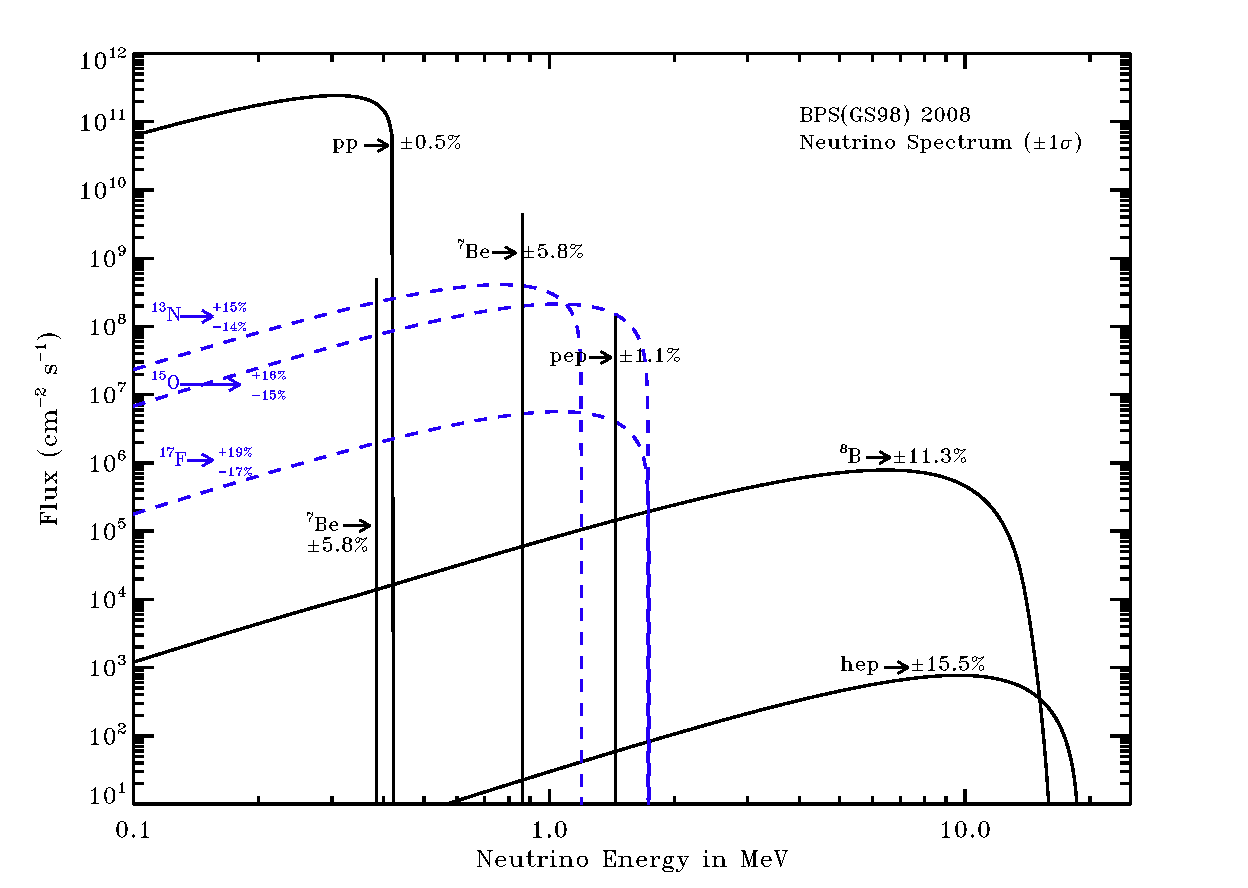
\includegraphics[width=0.6\linewidth]{figures/nu_spectrum1.pdf}
  \caption{
Solar neutrino spectra and SSM uncertainties \cite{serenellif}. 
}
 \label{fig:sol-spectra}
 \end{figure}


\begin{table}
\caption{Nuclear fusion reactions in the Sun and their neutrino fluxes (in units cm$^{-2}$ s$^{-1}$) according to the solar model GS98 \cite{serenelli}. The reactions in the last three lines are part of the CNO cycle.}
\centering
\begin{tabular}{|c|c|c|c|c|}
  \hline
  Reaction & $E_{MAX}$ (MeV) & GS98 & rel. unc. (\%) &name \\ 
  \hline
$ p + p \rightarrow {^2}H + e ^+ + \nu_e$ & 0.42 & 5.98    $10^{10}$ & 0.6 &pp \\
$ p + e^- + p \rightarrow {^2}H  + \nu_e$ & 1.44 & 1.44  $10^{8}$  & 1.2 &pep \\
$ {^7}Be + e^- \rightarrow {^7}Li + \nu_e$ & 0.86 & 5.00   $10^{9}$  & 7 &$ {^7}$Be \\
$ {^8}B \rightarrow {^8}Be + e ^+ + \nu_e$ & 15 & 5.58     $10^{6}$  & 14 &$ {^8}$B\\
$  {^3}He + p \rightarrow {^4}He + e ^+ + \nu_e$ & 18.77 & 8.04   $10^{3}$  & 30 &hep \\
$ {^{13}}N \rightarrow {^{13}}C + e ^+ + \nu_e$ & 1.2 & 2.96    $10^{8}$  &14  &$ {^{13}}$N\\
$ {^{15}}O \rightarrow {^{15}}N + e ^+ + \nu_e$ & 1.73 & 2.23     $10^{8}$  & 15& $ {^{15}}$O\\
$ {^{17}}F \rightarrow {^{17}}O + e ^+ + \nu_e$ & 1.74 & 5.52     $10^{6}$  & 16 &$ {^{17}}$F\\
  \hline
\end{tabular}
\label{tab:snuflux}
\end{table}


\subsection{The early experiments}

The radiochemical detection of neutrinos using the reaction 
$\nu_e~^{37}Cl\rightarrow~^{37}Ar~e^-$ was first suggested by Bruno Pontecorvo in 1946\cite{pontecorvo46}. This reaction has a threshold of 0.814 MeV and is therefore sensitive mainly to the $^8$B and $^8$Be solar neutrinos.

After previous experiments with this technique on surface, in 1965 Ray  Davis started  to construct a major experiment deep underground at Homestake (South Dakota), with 615~t of perchloroethylene (C$_2$Cl$_4$) that took data between 1968 and 2002.
The solar neutrino Argon production rate was 0.48 counts per day over a background of 0.09 counts per day due to the interactions initiated by highly energetic muons with nuclei (so called cosmogenics).
The $^{37}$Ar half-life of 35 days allows to expose the tank for a period of 60-70 days, followed by the efficient extraction of the produced argon purging the liquid with helium.  
The isotope $^{37}$Ar decays by electron capture: 90 \% of these occur on the K-shell producing an average of 3.5 Auger electrons with 2.82 keV of total energy. Miniature gas proportional counters were developed to detect with high efficiency and purity these decays, achieving single-atom counting.
The efficiency of the whole extraction chain was calibrated injecting know quantities of other argon isotopes.  

The result of the Homestake chlorine experiment~\cite{cleveland} for the capture rate  is
\begin{equation}
(\sigma \phi)_{Cl} = 2.56 \pm 0.16 \pm 0.16 SNU
\end{equation}
where SNU is Solar Neutrino Units (a SNU equals 10$^{-36}$ captures/nucleus/second) while the prediction from the solar model is $8.00 \pm 0.97$ SNU, that is the measured rate was approximately 30 \% of the predicted rate.  
Starting from the first result in 1968 this major deficit triggered a thirty years long debate, where many particle physicists were convinced that the reason of the discrepancies lied with the SSM. Indeed the rate of hydrogen burning depends critically on the temperature of the Sun core T as $T^{25}$ and helioseismological data were not yet available at that time to confirm the models. 

\begin{table}
\caption{Solar neutrino detectors. Verifier les masses}
\centering
\begin{tabular}{|c|c|c|c|c|c|}
  \hline
  Detector & Composition & Active mass & Threshold (MeV)  \\ 
  \hline
Homestake & C$_2$Cl$_4$ & 615t &  0.814 \\
Kamiokande & H$_2$O & 2.14kt &  7  \\
SAGE & Ga & 50t &  0.233 \\
GALLEX/GNO & Ga & 30.3t &  0.814  \\
Super-Kamiokande &  H$_2$O & 50kt &  3.5 \\
SNO & D$_2$O & 615 &  6\\
Borexino & C$_9$H$_{12}$ & 300t &  0.2  \\
  \hline
\end{tabular}

\label{tab:snudet}
\end{table}

It took more than twenty years before other radiochemical experiments could probe solar neutrinos. SAGE (1989-2007)~\cite{abdurashitov} in the Baksan Laboratory (Russia) and Gallex (1991-1997)~\cite{hampel}, followed by GNO (1998-2003)~\cite{altmann}, in the Gran Sasso Laboratory (Italy) used the reaction  $\nu_e ^{71} + Ga \rightarrow ^{71}Ge + e^-$
that has a low threshold, 0.233 MeV, and provides sensitivity to the pp neutrinos, constituting the majority of the flux. 

While the details of these experiments, related to the chemical properties of gallium, is different from Homestake, they follow that overall scheme of that experiment. They provided a confirmation of the solar neutrino deficit, although with a different reduction factor of approximately 50\% (Table~\ref{tab:snudet})~\cite{abdurashitov,hampel,altmann,kaether}:
\begin{eqnarray}
(\sigma \phi)_{SAGE} & = & 65.4^{+3.1} _{-3.0} ^{+2.6} _{-2.8}  SNU \\
(\sigma \phi)_{GALLEX} & = & 73.4  ^{+6.1}_{-6.0} ^{+3.7} _{-4.1} SNU \\
(\sigma \phi)_{GNO} & = & 62.9  ^{+5.5} _{-5.3} ^{+2.5} _{-2.5} SNU \\
\end{eqnarray}
to be compared to a predicted flux of 126.6 $\pm$ 4.2 SNU (GS98) (Fig.~\ref{fig:sol-theoryexp}).


\subsection{Real time experiments: Kamiokande, Super-Kamiokande, SNO, Borexino}

In 1987-1995 the 2.14 kt water Cherenkov experiment Kamiokande in Japan, in its phase II and III, provided a totally different measurement of the solar neutrinos. Neutrinos scattering on electrons, mainly sensitive to electron neutrinos, could be detected with a threshold of 9 MeV, progressively reduced to 7 MeV.  
The water Cherenkov technique, also used later by the Super-Kamiokande and the SNO experiments, will be described in section xx.   
Kamiokande was the first experiment to detect in real-time the solar neutrinos. Since the scattered electron is emitted preferentially in the direction of the neutrino, it could verify their solar origin by correlating the electron momentum with the Sun direction. The combined results~\cite{fukuda}
\begin{equation}
\phi( ^8 B) = [2.80 \pm 0.19 (stat) \pm 0.33 (sys)] \times 10^6 cm^{−2} s^{−1}
\end{equation}
or 50\% of the solar model prediction.

The 50kt water Cherenkov detector Super-Kamiokande, with a threshold of 7 MeV initially and today 3.5 MeV, started taking data in 1996 and confirmed the Kamiokande result with increased precision until its most recent update~\cite{abesk4}
\begin{equation}
\phi( ^8 B) = [2.308 \pm 0.020 (stat) ^{+0.040}_{-0.40} (sys)] × 10^6 cm^{−2} s^{−1}.
\end{equation} 

Super-Kamiokande is still running at present and it has recently observed for the first time a day-night effect for solar neutrinos~\cite{renshaw}. 
Let $r_D$ ($r_N$) be the day (night) event rate
the day-night asymmetry $A_{DN}$ is defined as $A_{DN} = \frac{2 (r_D - r_N) }{r_D + r_N}$ and was measured to be
\begin{equation}
A_{DN} = (−3.2 \pm 1.1 (stat) \pm 0.5 (syst)) \%,
\end{equation} 
deviating from zero by 2.7 $\sigma$.
This is the effect is similar to $K_S^0$ regeneration for a beam $K_L^0$ passing through a material. It is the first indication of matter effects on neutrino propagation. 


\begin{figure}[htbp]
\centering
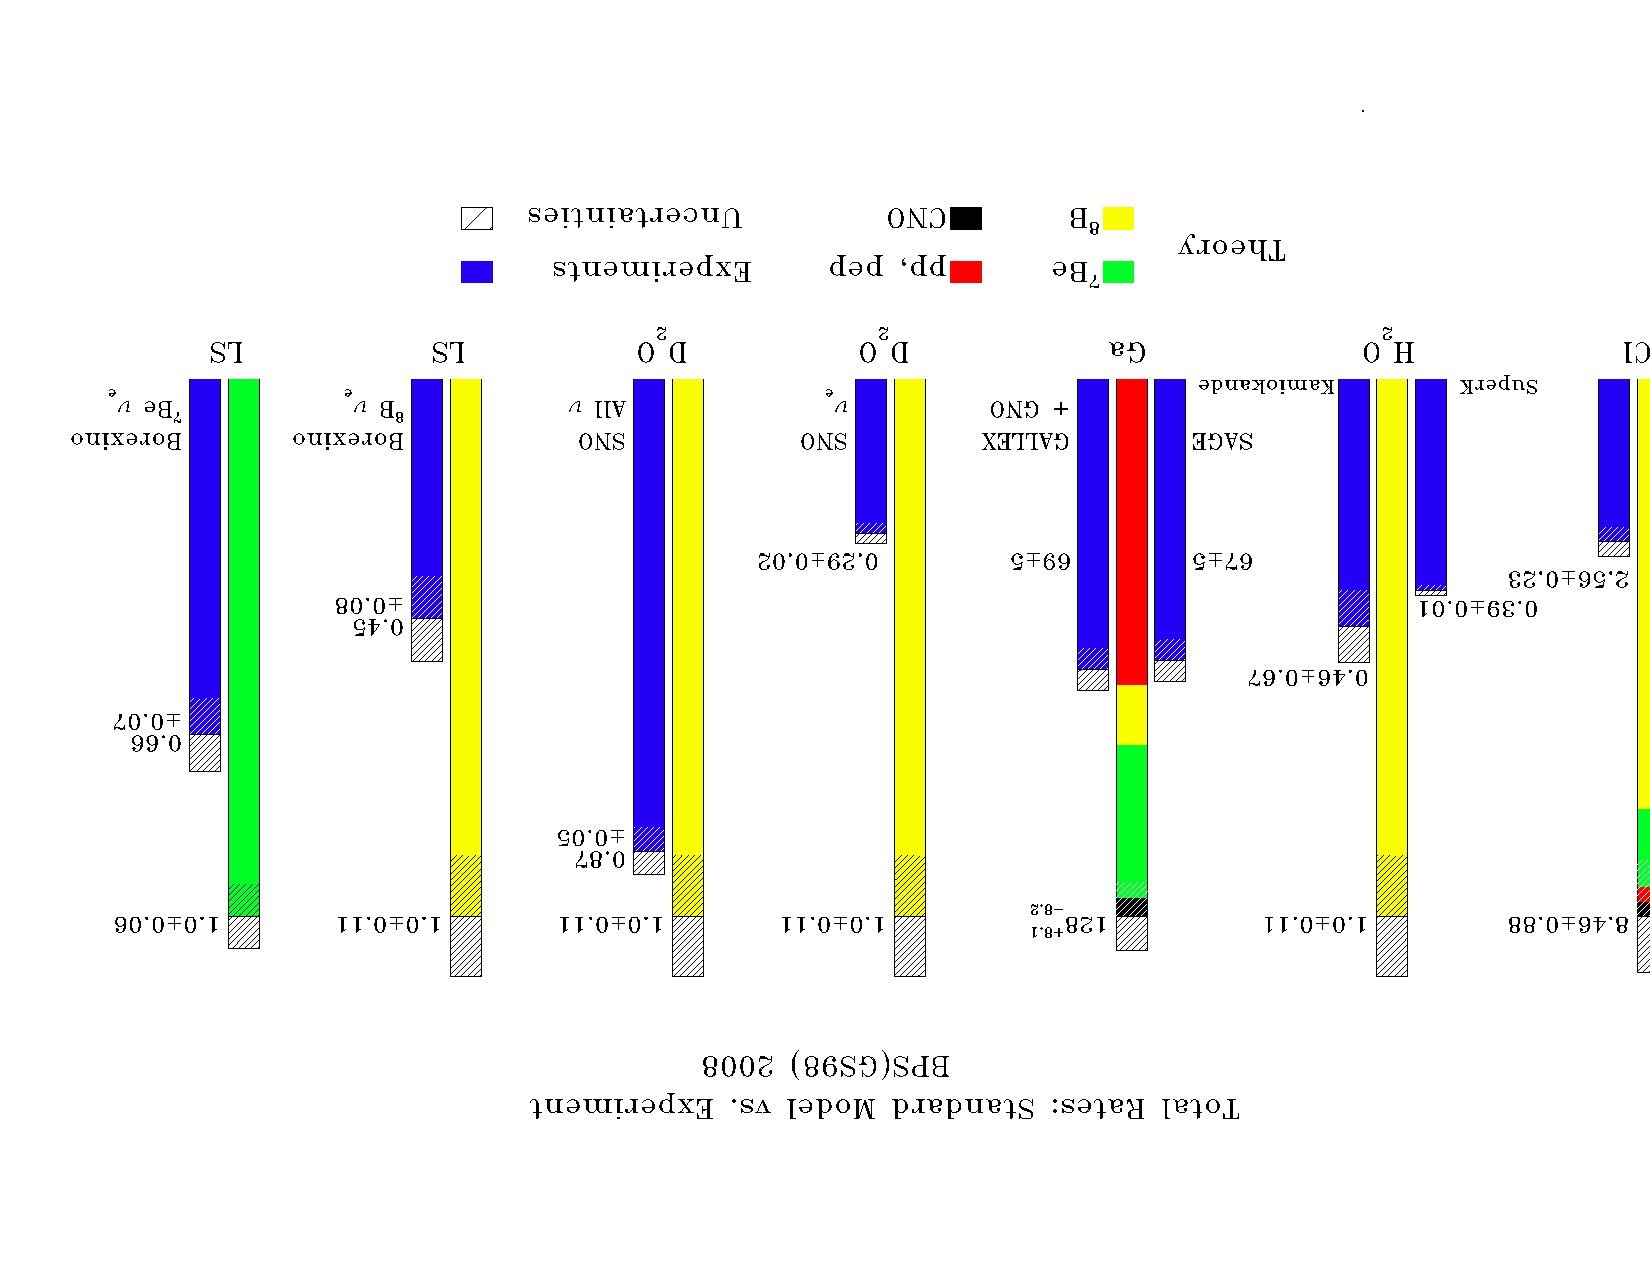
\includegraphics[angle=180,width=0.8\linewidth]{figures/theoryvsexpsnu1.pdf}
  \caption{
Measurements of the solar neutrino fluxes by various experiments compared to the SSM prediction~\cite{serenellif}.
}
 \label{fig:sol-theoryexp}
 \end{figure}



The real breakthrough came from the Sudbury Neutrino Observatory (SNO, Canada), a Cherenkov detector 2 km below ground containing 1~kt of heavy water. 
With heavy water, three channels are available to probe the solar neutrino flux: 
\begin{itemize}
\item The charged current reaction for electron neutrinos $ \nu_e + d \rightarrow p + p + e^−$, where the produced electron carry off most of the neutrino energy allowing to constrain the neutrino spectrum;
\item The neutral current reaction $ \nu_x + d \rightarrow \nu_x +  p + n $ which allow to count all the neutrinos, independently of their flavour, above the threshold of 2.22 MeV; 
\item The electron scattering (ES) reaction $ \nu_x + e^- \rightarrow \nu_x + e^−$ also available in conventional water Cherenkov detectors, which is mainly sensitive to $ \nu_e$, $\sigma_{ES}(\nu_e)\simeq 6 \sigma_{ES}(\nu_{\mu \tau})$. 
\end{itemize}
SNO took data in three phases, distinguished by the technique used to detect the neutron produced in the neutral current dissociation of deuterium. Indeed, as the neutron is the only detectable particle in this reaction, this measurement is an experimental challenge and places severe requirements on the radiopurity of the whole apparatus. In the first phase neutrons capture on deuterium was used. In the second phase, NaCl was dissolved in the water and neutrons were detected through the neutron capture on $^{35}$ Cl followed by gamma emission. In the third phase neutron detectors containing $^3$He were inserted in the detector.
The results of all phases of the detector were in agreement and yielded a measurement of the total flux of solar neutrinos~\cite{aharmim}, irrespective of their flavour,
\begin{equation}
\phi_{NC} (\nu active ) = [5.25 \pm 0.16 (stat) ^{+0.11}
_{-0.13} (syst)] \times
10^6 cm^{-2} s^{-1}$ 
\end{equation}
in agreement with the prediction of the solar models
and $\phi_{CC} (\nu_e ) =  0.301 \pm 0.033 \phi_{NC} (\nu active )$. As we will discuss in section
 \ref{subsec:solarinter} this is clearly an indication of flavour conversion for the solar neutrinos. 

Borexino(2007-present) is a 278~t liquid scintillator detector in the Gran Sasso Laboratory (Italy)
capable of measuring low energy neutrinos with a threshold of 200 keV in real time, thanks to the high light yield of 10$⁴$ photons per MeV which is much higher than in a Cherenkov detector. 
It measured the $^7$Be flux $(3.10 \pm 0.15) \times 10^9 cm^{-2} s^{-1}$ that is 62 \% of the GS98 SSM predicted flux~\cite{bellini}. It gave the first determination of the pep flux 
$(1.6 ± 0.3) \times 10^8 cm^{-2} s^{-1}$ and provided an upper limit on the CNO neutrino flux.


\subsection{Confirmation with artificial neutrinos: KamLAND}

KamLAND is a 1~kt liquid scintillator experiment located in the former site of the Kamiokande detector in Japan. As described in more detail in section xx, it is capable of detecting $\bar \nu_e$ emitted by nuclear reactors through the inverse beta decay reaction $\bar{\nu}_e p \rightarrow n e^+$. KamLAND is surrounded by 55 Japanese nuclear reactors at an average distance of 150 km. In 2002, it reported  evidence for the disappearance  of $\bar \nu_e$. In an updated report in 2008~\cite{kamland}, they observed 1609 
events to be compared to $2179 \pm 89$ expected from reactor neutrinos and  $276 \pm 23$ from background sources (Fig.~\ref{fig:sol-kam}). This measurement was decisive for the interpretation of solar neutrino data.

\begin{figure}[htbp]
\centering
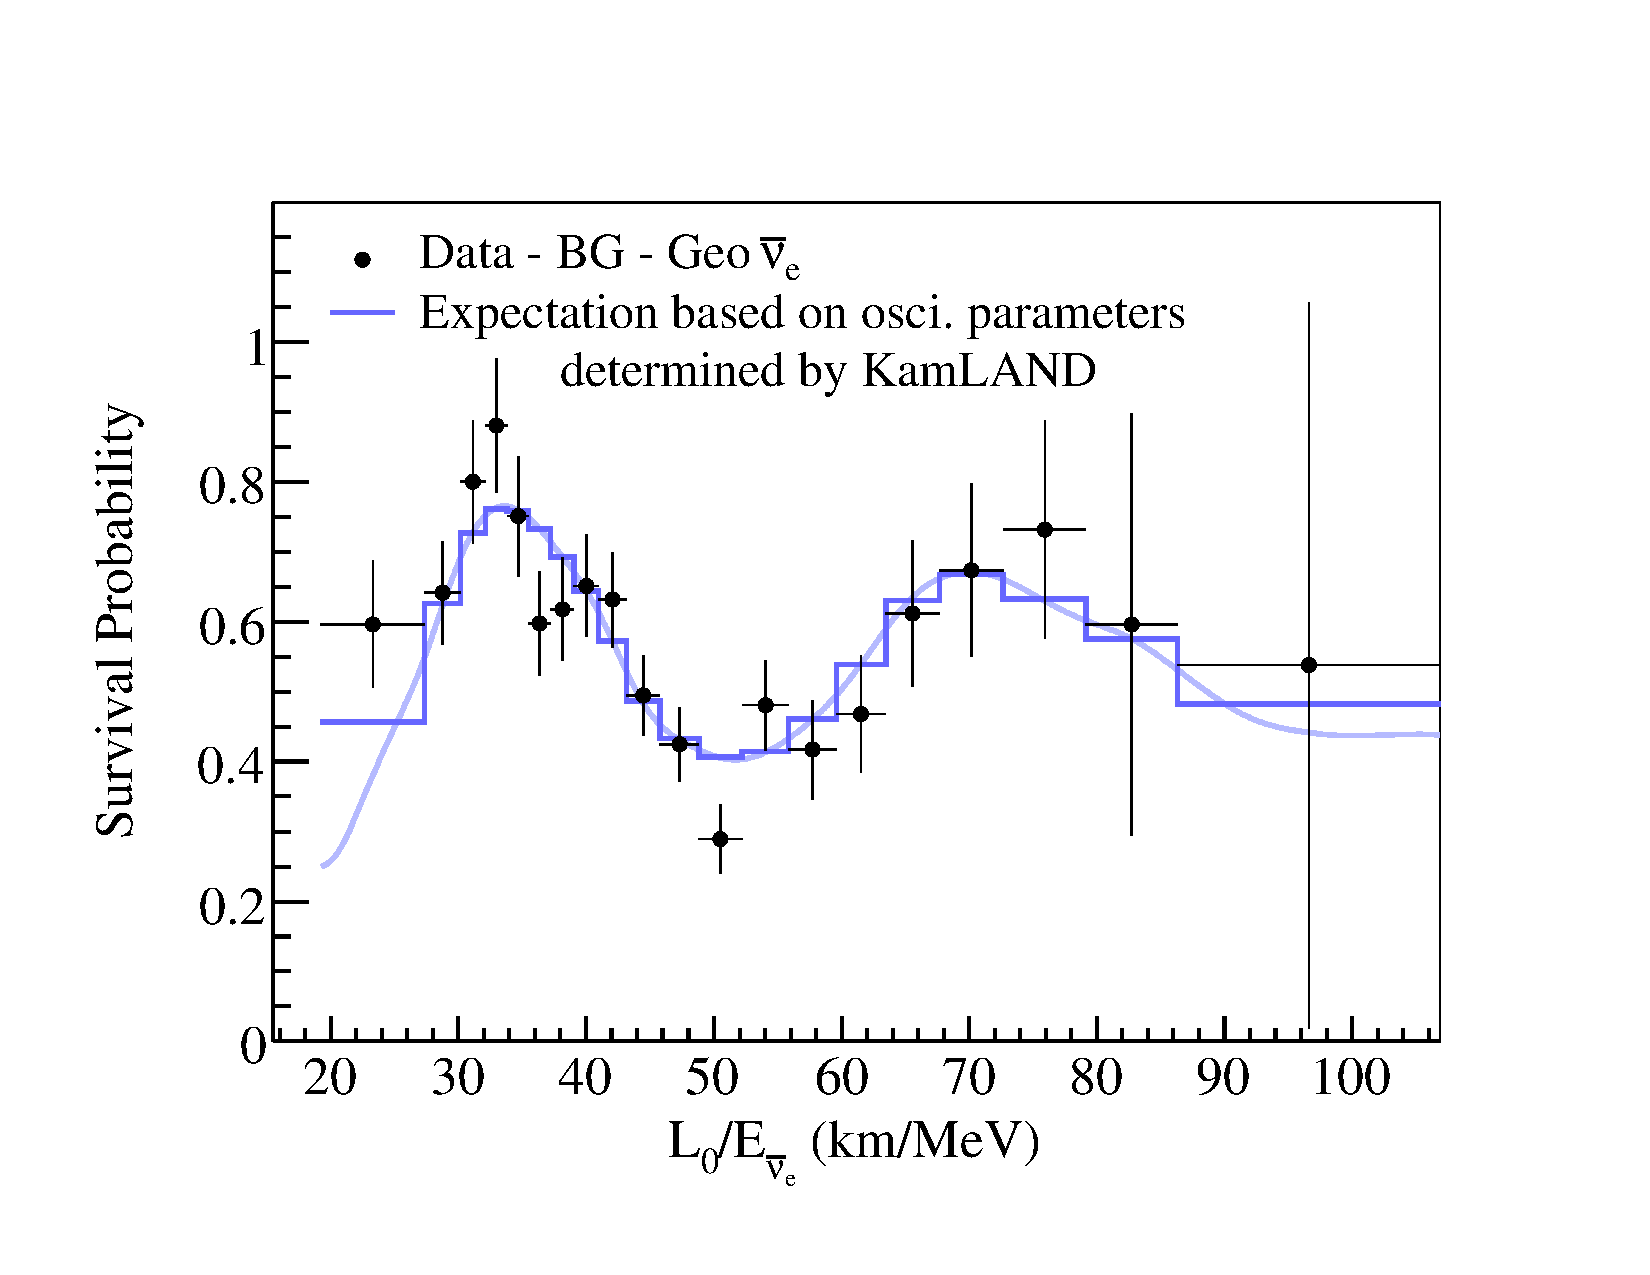
\includegraphics[width=0.6\linewidth]{figures/LE.pdf}
  \caption{KamLAND experiment: ratio of the background and geo-neutrino-subtracted $\bar{\nu}_e$
spectrum to the expectation for no-oscillation as a function of
L/E. The curve and histograms show the expectation for the best fit oscillation hypothesis.}
 \label{fig:sol-kam}
 \end{figure}



\subsection{Interpretation of the measurements and discussion}
\label{subsec:solarinter}
(MSW interpretation) Borexino  mesure various components of the spectrum (Be, CNO) $\rightarrow$ confirmation MSW (upturn) day night effect

The first measurement of a deficit of the solar neutrino flux left open several interpretations. While Pontecorvo made the hypothesis of neutrino oscillations, modest changes to the Sun core temperature could also be invoked. 
The situation changed with the new measurements by the gallium experiments, as it was clear that the suppression factor depended on the neutrino energy. The SNO results were the first measurement of the total solar neutrino flux and were also the first solid proof of flavour conversion as the explanation of the solar neutrino puzzle. 
Nevertheless, several different solutions were possible in term of the masses and mixing. The KamLAND result pinpointed one of them, the so-called Large Mixing Angle solution. Indeed, the results of KamLAND can be understood in term of a simple two neutrino mixing formula $ P(\bar{\nu}_e \rightarrow \bar{\nu}_e ) = 1 - \sin^2 (2 \theta_{12}^2) \sin^2 \frac{\Delta m^2_{21} L}{4 E} $, neglecting matter effects and effects related to $\theta_{13}$. As we will see later, the value of $\Delta m^2_{31}$ is much larger than $\Delta m^2_{21}$ and induces rapid oscillations that are averaged out given the $L$, $E$ and energy resolution of that experiment. The $L/E$ pattern is prominent in the KamLAND data and beautifully confirms neutrino oscillations as the origin of their observed deficit (Fig.~\ref{fig:sol-kam}). The measurement of KamLAND allows to determine $\Delta m^2_{21} = (7.59 \pm 0.21) 10^{-5}
eV^2$ and $\tan^2 \theta^{12} = 0.47 ^{+0.06} _{−0.05} $.

The explanation of the deficit observed by the solar neutrino experiments involves flavour transitions of a different kind. As explained in section xx, electron neutrinos are produced in the center of the Sun in a medium of high density. If the condition $n \gt n_{res}$, or $ n \gt \frac{\Delta m^2_{21} \cos 2 \theta_{12}}{ 2 \sqrt{2}G_F E}$ is satisfied, corresponding to energies above 1.9 (verifier 5 intro????) MeV, neutrinos are produced as the $ \nu^m_2$ matter eigenstates of the Hamiltonian and in its adiabatic evolution exits the Sun as $\nu_2$. The probability to observe them as $\nu_e$ is then $\sin^ \theta_{12}$. For neutrinos produced with energies much below this threshold, matter effect can be neglected and they undergo vacuum oscillations. The suppression factor is then the result of the averaging of many oscillation periods    
$ P({\nu}_e \rightarrow {\nu}_e ) = 1 - \frac{1}{2} \sin^2 (2 \theta_{12}^2)$. 
It can be shown that for neutrino energies far above the resonance condition the adiabatic condition does not hold any more and that the suppression factor is $\cos^2 \theta_{12} $. This leads to a characteristic "bath tub" shape for the neutrino survival probability. This interpretation fits with all the solar neutrino data (add figure). 













